\documentclass[a4paper, titlepage]{article}
%Not used in XeTeX, is used in pdfTex
\usepackage[utf8]{inputenc}
\usepackage{booktabs} % Nice tables
\usepackage{tabulary} % Also nice tables
\usepackage{3parttable} % Tables with footnotes
\usepackage{caption} % required for above
\usepackage{hyperref} % Hyperlinks, hyperlinks everywhere
\usepackage{graphicx} % Pics or it didn't happen...
\usepackage{minted} % Look at the pretty colours, and indenting, and wrapping...

\def\sectionautorefname{Section}
\def\subsectionautorefname{Subsection} % Reassing the default names to have capitals.

\captionsetup{justification=raggedright, singlelinecheck=false, format=hang}
\newcommand{\gref}[1]{\hyperref[#1]{\autoref*{#1}: \nameref{#1}}} % Good referencing = gref



\begin{document}
	\title{F28DM - Coursework 1}
	\author{{\Large Group ED1}\\\\Tommy Lamb\\ Daniel Banister\\ Daniel Barker}
	\maketitle
	\tableofcontents
	\clearpage
	
	\section{Scenario and Conceptual Model} \label{sec:scenario}
	\subsection{Extended Scenario}
	The sports centre offers various levels of membership, with each level having different prices based on Monthly or Annual payments. The sports centre allows members to automatically renew their membership, but also keeps their details after their membership expires, to allow them to advertise special deals enticing them to return. Members are not allowed to share their memberships IE no family deals. Each member will have a unique ID number, associated with their name, date of birth, email, and telephone details. The database should also track the length of their  membership (date started and expiration date) alongside whether the membership has expired and whether the customer set their membership to automatically renew.
	\\\\
	Each member is allowed to book the use of either an entire room (and all of its equipment) or for specific pieces of equipment. Since some members have their own equipment (racquets for example) not all bookings will require a piece of gym-owned equipment to be booked. Some pieces of equipment require special training before they can be used by members, and there must always be a member of staff who has passed the course for any piece of equipment. When a member makes a room booking they must have relevant training for all the equipment in that room. Some training courses will have multiple levels associated with them which need to be individually tracked. The sports centre also wishes to track if training courses are accredited by outside organisations, such as Cycling Scotland. Even when booking only a generic piece of equipment e.g. treadmill members will be given a specific room to use. Though members may make multiple bookings, they may not overlap. Each booking will have its own unique ID code and will store the date and start- and end-times of the booking, as well as recording if the booking is for a whole room. 
	\\\\
	To promote a healthy workplace all staff who work for the sports centre are automatically given free memberships, the level of which is associated with their pay grade which depends on their position and length of service within the company, which need to be recorded. All staff members also have a supervisor to whom they report, with the exception of the General Manager. The database will also need to store the Staff passwords to allow them access to the booking system, as well as holding information about the various pay grades, including the salary and associated membership level, to enforce staff benefits.
	\\\\
	The facilities manager requires the ability to track the various different pieces of equipment in the centre, as over the years the inventory has become fragmented with various different models and variations of specific equipment. For example, the centre has 3 different treadmill models in inventory and climbing walls of various difficulty. Periodically the manager will scrap or sell older models, or add newer equipment to the inventory. Because of the diversity of activities offered by the centre the database will only store the type of a piece of equipment (e.g. Treadmill) and some undefined identification (e.g. "Windwalker 200", "Olympic Size"). Alongside this the database is to record how much of each piece of equipment there is, and which rooms they are in. Due to health and safety laws each room has a maximum limit on the number of occupants, which does not necessarily correlate with the amount of equipment in each and must be stored to ensure no rooms are overbooked.  
	
	\subsection{ER Diagram}
	The image can be found full size \href{https://drive.google.com/file/d/0B1dD0VdrKINebGRlLVN0OFhrQ2c/view?usp=sharing}{\underline{here}}\\
	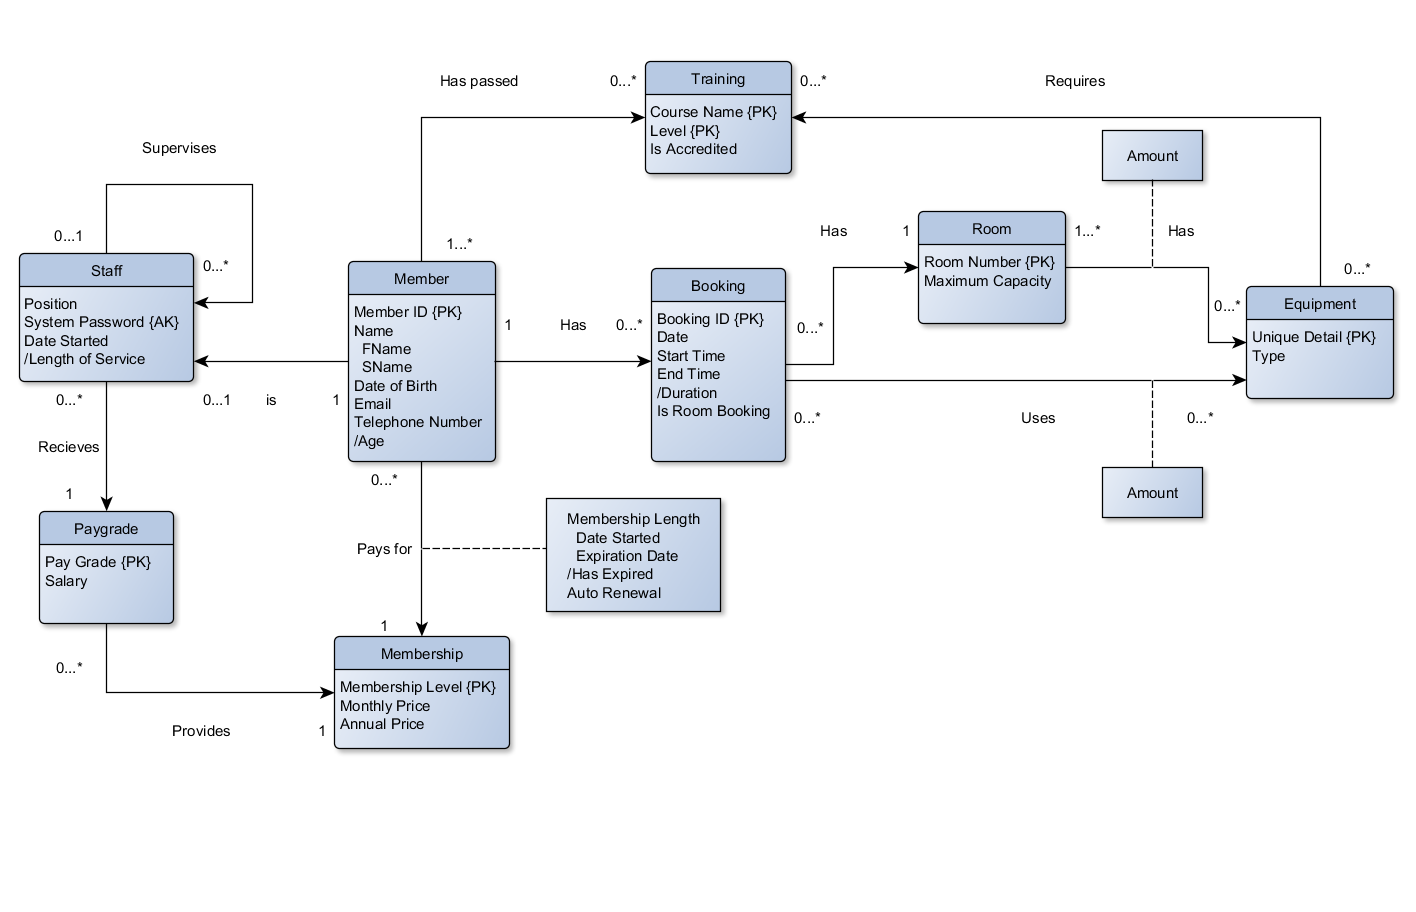
\includegraphics[scale=0.32]{ERDiagram}
	
	
	\section{Relational Schema} \label{sec:schema}
		
	\subsection{Data Dictionaries}
	
	%Staff
	\begin{threeparttable}
	\begin{tabulary}{1.2\textwidth}{ l L l l l l }
	
		\multicolumn{6}{ >{\bfseries \large} l}{Staff}\\ \midrule
		Attribute & Description & Domain & Nullable & Primary Key & Foreign Key \\ \midrule
		mID & The unique ID number given to all sports centre members & Int(8) & No & Yes & Yes \\
		position & The position a staff member holds within the company, eg facilities manager & Text(24) & No & No & No \\
		pword & The password used by staff to log on to the System. Hashed. & Text(256)\tnote{a} & No & No & No \\
		sStarted & The date a staff member started working for the sports centre & Date & No & No & No \\ 
		supMID & The membership ID of a staff member's supervisor & Int(8) & Yes & No & Yes \\
		paygrade & The paygrade of a staff member & Text(2) & No & No & Yes \\
		\bottomrule
		
	\end{tabulary}
	\begin{tablenotes}
		\item[a] Size required to ensure scalability with future hashing algorithms  
	\end{tablenotes}
	\end{threeparttable}

	%Member
	\begin{threeparttable}
	\begin{tabulary}{1.2\textwidth}{ l L l l l l }
		
		\multicolumn{6}{ >{\bfseries \large} l}{Member}\\ \midrule
		Attribute & Description & Domain & Nullable & Primary Key & Foreign Key \\ \midrule
		mID & The unique ID number given to all sports centre members & Int(8) & No & Yes & No \\
		fNames & The first and middle names of a member & Text(32) & No & No & No \\
		sName & The surname of a member & Text(32) & No & No & No \\
		dob & The date of birth of a member & Date & No & No & No \\ 
		email & The email address of a member & Text(256)\tnote{a} & Yes & No & No \\
		tNumber & The telephone number of a member & Text(11)\tnote{b,c} & No & No & No \\
		mLevel & The membership level a member holds & Int(2) & No & No & Yes \\
		mStarted & The date a member's membership began & Date & No & No & No \\
		mExpire & The date the membership will expire & Date & No & No & No \\
		autoRenew & Whether the membership will automatically renew or not & Boolean & No & No & No\\
		\bottomrule
		
	\end{tabulary}
	\begin{tablenotes}
		\item[a] Size determined by reference to RFC 5321. SMTP forward and reverse paths are up to 256 characters long.
		\item[b] Only standard British landline and mobile numbers are considered in scope.
		\item[c] Stored as text to maintain any leading zeroes.
	\end{tablenotes}
\end{threeparttable}
	
	\vspace{1cm}
	%Booking
		\begin{tabulary}{1.2\textwidth}{l L llll}
			\multicolumn{6}{ >{\bfseries \large} l}{Booking}\\ \midrule
			Attribute & Description & Domain & Nullable & Primary Key & Foreign Key \\ \midrule
			bID & ID number for specific booking & Int(8) & No & Yes & No \\
			mID & ID number for member who made the booking & Int(8) & No & No & Yes \\
			rNumber & Room number of the booking & Int(4) & No & No & Yes \\
			date & The date of the booking & Date & No & No & No \\
			sTime & The time the booking starts & Time & No & No & No \\
			eTime & The time the booking ends & Time & No & No & No \\
			isRoomBooking & Flag if the booking is for an entire room & Boolean & No & No & No \\ \bottomrule
		\end{tabulary}


	
		%Room
\vspace{1cm}
	\begin{tabulary}{1.2\textwidth}{l L llll}
		\multicolumn{6}{ >{\bfseries \large} l}{Room}\\ \midrule
		Attribute & Description & Domain & Nullable & Primary Key & Foreign Key \\ \midrule
		rNumber & Unique room number & Int(4) & No & Yes & No \\
		capacity & Maximum amount of people allowed in a room at any given time & Int(4) & Yes & No & No \\
		\bottomrule
	\end{tabulary}


\vspace{1cm}
	%Equipment
	\begin{tabulary}{1.2\textwidth}{l L llll}
		\multicolumn{6}{ >{\bfseries \large} l}{Equipment}\\ \midrule
		Attribute & Description & Domain & Nullable & Primary Key & Foreign Key \\ \midrule
		detail & A unique identifying detail e.g. Model name and number & Text(64) & No & Yes & No \\
		type & The type of a piece of equipment e.g. Treadmill & Text(24) & No & No & No \\
		\bottomrule
	\end{tabulary}

\vspace{1cm}
%Membership
\begin{tabulary}{1.2\textwidth}{l L llll}
	\multicolumn{6}{ >{\bfseries \large} l}{Membership}\\ \midrule
	Attribute & Description & Domain & Nullable & Primary Key & Foreign Key \\ \midrule
	mLevel & An arbitrary number representing the level of membership & Int(2) & No & Yes & No \\
	mPrice & The monthly price of this membership level& Decimal(5,2) & No & No & No \\
	aPrice & The annual price of this membership level & Decimal(5,2) & No & No & No \\
	\bottomrule
\end{tabulary}

\vspace{1cm}
%Training
\begin{tabulary}{1.2\textwidth}{l L llll}
	\multicolumn{6}{ >{\bfseries \large} l}{Training}\\ \midrule
	Attribute & Description & Domain & Nullable & Primary Key & Foreign Key \\ \midrule
	cName & The name of the course & Text(24) & No & Yes & No \\
	tLevel & Arbitrary number representing difficulty of course & Int(2) & No & Yes & No \\
	isAccredited & Records if this course is accredited by an external organisation & Boolean & No & No & No \\
	\bottomrule
\end{tabulary}

\vspace{1cm}
%Paygrade
\begin{tabulary}{1.2\textwidth}{l L llll}
	
	\multicolumn{6}{ >{\bfseries \large} l}{Paygrade}\\ \midrule
	Attribute & Description & Domain & Nullable & Primary Key & Foreign Key \\ \midrule
	paygrade & Code representing employee salary and benefits on an arbitrary scale & Text(2) & No & Yes & No \\
	salary & Payment amount received by staff on this pay grade & Decimal(8,2) & No & No & No \\
	mLevel & The level of free membership provided & Int(2) & No & No & Yes \\
	\bottomrule
\end{tabulary}

%HasPassed
\vspace{1cm}
\begin{tabulary}{1.2\textwidth}{l L llll}
	\multicolumn{6}{ >{\bfseries \large} l}{HasPassed}\\ \midrule
	Attribute & Description & Domain & Nullable & Primary Key & Foreign Key \\ \midrule
	mID & ID number of member & Int(8) & No & Yes & Yes \\
	cName & Name of course passed by member & Text(32) & No & Yes & Yes \\
	tLevel & The level of course passed & Int(2) & No & Yes & Yes \\
	\bottomrule
\end{tabulary}

%Requires
\vspace{1cm}
\begin{tabulary}{1.2\textwidth}{l L llll}
	\multicolumn{6}{ >{\bfseries \large} l}{Requires}\\ \midrule
	Attribute & Description & Domain & Nullable & Primary Key & Foreign Key \\ \midrule
	detail & Unique detail of the equipment & Text(64) & No & Yes & Yes \\
	cName & Name of course passed by member & Text(32) & No & Yes & Yes \\
	tLevel & The level of course passed & Int(2) & No & Yes & Yes \\
	\bottomrule
\end{tabulary}

%Has
\vspace{1cm}
\begin{tabulary}{1.2\textwidth}{l L llll}
	\multicolumn{6}{ >{\bfseries \large} l}{Has}\\ \midrule
	Attribute & Description & Domain & Nullable & Primary Key & Foreign Key \\ \midrule
	rNumber & Room number storing the related equipment & Int(4) & No & Yes & Yes \\
	detail & Unique detail of the equipment stored & Text(64) & No & Yes & Yes \\
	amount & The amount of the equipment being stored & Int(4) & No & No & No \\
	\bottomrule
\end{tabulary}


%Uses
\vspace{1cm}
\begin{tabulary}{1.2\textwidth}{l L llll}
	\multicolumn{6}{ >{\bfseries \large} l}{Uses}\\ \midrule
	Attribute & Description & Domain & Nullable & Primary Key & Foreign Key \\ \midrule
	bID & ID of the booking in question & Int(8) & No & Yes & Yes \\
	detail & Unique detail of the equipment booked & Text(64) & No & Yes & Yes \\
	amount & The amount of the equipment being booked & Int(4) & No & No & No \\
	\bottomrule
\end{tabulary}

\section{Schema Implementation}
All comments on the implementation of the schema in MySQL can be found in the SQL script file as requested. This section is included here to allow the section numbering to match that of the coursework specification, minimising confusion.


\section{Loading Data} \label{sec:data}
\subsection{Bulk Loader and INSERT}
As the name would suggest, the bulk loader was reserved for large volumes of largely homogeneous data, the kind which could be generated easily by computer scripts, while other more bespoke data was handled through \mintinline{sql}{INSERT} statements. While some of the data may seem facetious the exact content is largely unimportant for this purpose, such as the name of equipment or training courses. If anything, such distinctive data makes testing easier, as one becomes more familiar with the data than if it were bland, boring, or normal.
\\
Note that the membership start dates were randomly modified after loading them into the database to rectify the fact that they all started on 2017/02/25 and as such are not replicable. This date entry was initially chosen to mimic the query as it would be used if the system was complete: automatically determining mStarted as the date they were entered into the DB. All other pertinent data is replicable however.
\\ \\
The following data was loaded through the Bulk Loader:
\begin{itemize}
	\item Equipment (excluding Climbing Walls)
	\item Training (excluding "Rock Climbing")
	\item Staff Members (both Staff and Member tables)
	\item Non-staff Members (both with and without email addresses)
	\item Members' Training (HasPassed table)
\end{itemize}
\ \\
The following was loaded using \mintinline{sql}{INSERT} statements.
\begin{itemize}
	\item All Membership values
	\item All Paygrade values
	\item "Rock Climbing" training course
	\item "Climbing Wall" equipment types
	\item All Requires table values
	\item All Room table values
	\item All Has table values
	\item Staff member "Sir Topham Hatt" (Staff and Member tables)
	\item Non-staff member "Garrus Vakarian"
	\item Member Garrus' training "Rock Climbing"
	\item Staff Member mID 5 training "Rock Climbing"
	\item All Booking table values
	\item All Uses table values
\end{itemize}

\subsection{Example Data}
	\begin{tabulary}{1.2\textwidth}{ l l l l l l }
		\multicolumn{6}{ >{\bfseries \large} l}{Member}\\ \midrule
		mID & fNames & sName & dob & email & tNumber \\ \midrule
		2 & Edward & Dee & 2010-05-11 & Edward@cameron.com & 07700900151 \\
		5 & James & Forth & 1990-11-28 & NULL & 07700900798 \\
		782 & Garrus & Vakarian & 2007-11-20 & archangel@omegaextra.net & 07700900856 \\
		122 & Dorothy & Wheeler & 1917-07-18 & dwheeler2y@theglobanadmail.com & 08368290528 \\
		\midrule
		mLevel & mStarted & mExpire & autoRenew \\
		3 & 2017-02-24 & 2018-02-24 & 1 \\
		2 & 2017-02-24 & 2018-02-23 & 1 \\
		2 & 2017-02-24 & 2017-03-23 & 1 \\
		1 & 2017-02-24 & 2017-03-24 & 0\\
		\bottomrule
\end{tabulary}
\vfill
\begin{tabulary}{1.2\textwidth}{ l l l l l l}
	\multicolumn{6}{ >{\bfseries \large} l}{Staff}\\ \midrule
	mID & position & pword & sStarted & supMID & paygrade \\ \midrule
	2 & Manager & \$2a\$07\$DDJaLGI ... & 2017-02-04 & NULL & A3 \\
	5 & Facilites & \$2a\$07\$2vebY ... & 2017-02-24 & 1 & D2 \\
	3 & DBA & \$2a\$07\$pKi2 ... & 2017-02-24 & 1 & B3 \\
	\bottomrule
\end{tabulary}

\vspace{1cm}
\begin{tabulary}{1.2\textwidth}{ l l l }	
	\multicolumn{3}{ >{\bfseries \large} l}{Paygrade}\\ \midrule
	paygrade & salary & mLevel \\ \midrule
	A3 & 45500.00 & 3 \\
	B3 & 30000.00 & 3 \\
	D2 & 18650.00 & 2 \\
\bottomrule
\end{tabulary}

\vspace{1cm}
\begin{tabulary}{1.2\textwidth}{ l l l }	
	\multicolumn{3}{ >{\bfseries \large} l}{Membership}\\ \midrule
	mLevel & mPrice & aPrice \\ \midrule
	1 & 10.00 & 100.00 \\
	2 & 27.50 & 288.00 \\
	3 & 33.33 & 366.00 \\
	\bottomrule
\end{tabulary}

\vspace{1cm}
\begin{tabulary}{1.2\textwidth}{ l l l }	
	\multicolumn{3}{ >{\bfseries \large} l}{HasPassed}\\ \midrule
	mID & cName & tLevel \\ \midrule
	2 & Rock Climbing & 2 \\
	5 & Classical Education & 2 \\
	5 & Rock Climbing & 4 \\
	122 & Classical Education & 2\\
	782 & Rock Climbing & 5 \\
	782 & Classical Education & 2 \\
	53 & Football Referee & 1 \\
	\bottomrule
\end{tabulary}

\vspace{1cm}
\begin{tabulary}{1.2\textwidth}{ l l l }	
	\multicolumn{3}{ >{\bfseries \large} l}{Training}\\ \midrule
	cName & tLevel & isAccredited \\ \midrule
	Classical Education & 2 & 0 \\
	Rock Climbing & 2 & 0 \\
	Rock Climbing & 4 & 1 \\
	Football Referee & 1 & 0 \\
	GB Spotters & 2 & 1 \\
	\bottomrule
\end{tabulary}

\vspace{1cm}
\begin{tabulary}{1.2\textwidth}{ l l l }	
	\multicolumn{3}{ >{\bfseries \large} l}{Requires}\\ \midrule
	detail & cName & tLevel \\ \midrule
	Realistic Rockface & Rock Climbing & 5 \\
	Realistic Rockface & Classical Education & 1 \\
	50M Overhang & Rock Climbing & 3 \\
	Outdoor Competition Size Grass & Football Referee & 4\\
	Oxford & Classical Education & 2 \\
	\bottomrule
\end{tabulary}

\vspace{1cm}
\begin{tabulary}{1.2\textwidth}{ l l }	
	\multicolumn{2}{ >{\bfseries \large} l}{Equipment}\\ \midrule
	detail & type \\ \midrule
	Realistic Rockface & Climbing Wall \\
	50M Overhang & Climbing Wall \\
	Oxford & Rowing Machine \\
	Outdoor Competition Size Grass & Football Pitch \\
	Specialized & Spinning Bike \\
	Python 3 & Treadmill \\
	Prolog & Treadmill \\
	Poly/ML & Treadmill \\	
	\bottomrule
\end{tabulary}

\vspace{1cm}
\begin{tabulary}{1.2\textwidth}{ l l l }	
	\multicolumn{3}{ >{\bfseries \large} l}{Has}\\ \midrule
	rNumber & detail & amount \\ \midrule
	1 & 50M Overhang & 2 \\
	1 & Realistic Rockface & 1 \\
	2 & Prolog & 7 \\
	4 & Specialized & 8 \\
	4 & Boardman & 8 \\
	5 & Cambridge & 3 \\
	5 & Oxford & 8 \\
	11 & Outdoor Competition Size Grass & 1 \\
	\bottomrule
\end{tabulary}

\vspace{1cm}
\begin{tabulary}{1.2\textwidth}{ l l }	
	\multicolumn{2}{ >{\bfseries \large} l}{Room}\\ \midrule
	rNumber & capacity \\ \midrule
	1 & 40 \\
	2 & 20 \\
	4 & 20 \\
	5 & 10 \\
	11 & NULL \\
	\bottomrule
\end{tabulary}

\vspace{1cm}
\begin{tabulary}{1.2\textwidth}{ l l l l l l l }	
	\multicolumn{3}{ >{\bfseries \large} l}{Booking}\\ \midrule
	bID & mID & rNumber & date & sTime & eTime & isRoomBooking \\ \midrule
	2 & 2 & 1 & 2017-02-25 & 11:00:00 & 12:00:00 & 0 \\
	1 & 782 & 1 & 2017-02-25 & 12:00:00 & 14:00:00 & 0 \\
	3 & 23 & 1 & 2017-02-25 & 13:00:00 & 13:30:00 & 0 \\
	8 & 782 & 4 & 2017-02-25 & 15:00:00 & 17:00:00 & 1 \\
	9 & 554 & 7 & 2017-02-25 & 12:00:00 & 16:00:00 & 1 \\
	7 & 122 & 5 & 2017-02-25 & 09:00:00 & 12:00:00 & 0 \\
	6 & 203 & 1 & 2017-02-26 & 14:00:00 & 15:00:00 & 0 \\
	\bottomrule
\end{tabulary}

\vspace{1cm}
\begin{tabulary}{1.2\textwidth}{ l l l }	
	\multicolumn{3}{ >{\bfseries \large} l}{Uses}\\ \midrule
	bID & detail & amount \\ \midrule
	1 & 50M Overhang & 1 \\
	2 & 100M Vertical & 1 \\
	3 & 50M Overhang & 1 \\
	6 & Realistic Rockface & 1 \\
	7 & Cambridge & 3 \\
	7 & Oxford & 5 \\
	8 & Boardman & 8 \\
	8 & Specialized & 8 \\
	\bottomrule
\end{tabulary}

\section{Roles, Permissions, and Views} \label{sec:roles}
\subsection{Roles and Permissions}
For the purposes of this section, and since MySQL 5.6 doesn't support roles, a user account was created for each envisioned role within the sports centre. These user accounts were defined in such a way that multiple end users could use the same account for database access (simulating roles), achieved by using an undefined desktop app. Since very few staff end users would actually know SQL, the use of an application is a realistic scenario. This external application would deal with verifying the credentials of individual end users, while the database system manages security for groups of end users. The groups that were identified were:
\begin{itemize}
	\item DB Administrators
	\begin{itemize}
		\item Senior IT employees in charge of administering the Database, trusted with access to all data in the database without constraint.
		\item Also have access to the IT user account to allow some remote administration.
	\end{itemize}
	\item Human Resources
	\begin{itemize}
		\item HR are in charge of all members of staff. They do not however have access to the hashed passwords of staff, or to the details of non-staff members of the centre. They can also view, but not change, paygrade information.
		\item DB Row-wise restrictions on HR end users would be implemented at the application level, such that HR staff cannot change their own pay grade or other details.
	\end{itemize}
	\item Finance
	\begin{itemize}
		\item The department in charge of setting pay grades, and membership levels and pricing. Though they set the salary and membership level associated with each pay grade, they do not dictate directly the pay of a member of staff.
	\end{itemize}
	\item Facilities
	\begin{itemize}
		\item As the name suggests, Facilities is in charge of all of the rooms and equipment within the sports centre. This includes setting the training required by any piece of equipment. 
		\item The dept. also has access to an anonymised list of members and the equipment they are trained for, as well as contact information for all staff members. This allows the constraint that every piece of equipment must have a staff member trained on it be checked, and amongst other things, data-driven decisions.
	\end{itemize}
	\item Customer Services
	\begin{itemize}
		\item A large department with far-reaching read access, Customer Services are in charge of all bookings, training, and the details of all non-staff members. This department can create new training courses, but cannot remove them due to the "equipment requires training" relationship to which they have limited access.
		\item While the Dept. can view the details of staff members from the Member table to administer staff bookings, they have no access to the Paygrade or Staff tables.
	\end{itemize}
	\item IT
	\begin{itemize}
		\item In charge of all computing equipment in the centre, IT has a large range of permissions over all tables, with some limitations. For example the permission to drop tables and certain other administrative commands are limited to DBAs, and they also have limited permissions on the Staff and Paygrade tables to prevent misuse.
	\end{itemize}
\end{itemize}
Since online bookings were not specified, a user account was not created to enable them; rather all bookings are made through the Customer Service department. Further to this, the database is only accessible from within the LAN as a security precaution, with each user group operating from within a specific subnet of the LAN. DB Administrators are an exception to this however, as their all-powerful \mintinline{sql}{root} account is only valid when accessing the database from \mintinline{sql}{localhost}. The IT user account can be accessed from any subnet to allow on-site assistance.

\subsection{Views}

Due to the ability to set certain permissions on a column basis, views have largely been used as a tool of simplification rather than security. Predominately abstracting over table joins, they make the granting of permissions and complex queries somewhat simpler; they also enable the differentiation between staff members and non-staff members within the \mintinline{sql}{Member} table, impossible with pure permissions. 
\\
All of the following views are created using the MySQL default security mode, checking the permissions of the view definer rather than the user account referencing the view for the underlying tables; all user accounts still require adequate permissions on the view itself. Where views can be updated or inserted to, it is subject to the constraints described in the MySQL 5.6 documentation: \href{https://dev.mysql.com/doc/refman/5.6/en/view-updatability.html}{20.5.3 Updatable and Insertable Views}. Due to their possible usage for insertion or updating, all relevant views implement the \mintinline{sql}{WITH CHECK OPTION} option.
\begin{itemize}
	\item ViewStaffMembers
	\begin{itemize}
		\item A view which selects only the rows from \mintinline{sql}{Member} which represent staff members. Used to enable permissions to be set for only staff members.
		\item Returns all columns.
		\item Is used in granting permissions.
		\item Can update, insert to, and delete from.
	\end{itemize}
	\item ViewNonStaffMembers
	\begin{itemize}
		\item The inverse of the previous view, this selects all rows for which the membership number \mintinline{sql}{mID} does not represent a staff member. Used to enable permissions to be set for only non-staff members.
		\item Returns all columns.
		\item Is used in granting permissions.
		\item Can update, insert to, and delete from.
	\end{itemize}
	\item ViewMemberTraining
	\begin{itemize}
		\item A view to abstract over the joining of the \mintinline{sql}{Training} and \mintinline{sql}{HasPassed} tables.
		\item Returns membership number,training name, level and \mintinline{sql}{isAccredited}.
		\item Is used in permissions
		\item Can update and insert to, but not delete from. 
	\end{itemize}
	\item ViewEquipmentTraining
	\begin{itemize}
		\item Simply joins the \mintinline{sql}{Equipment} and \mintinline{sql}{Training} tables through the \mintinline{sql}{Requires} linking table. Used to simplify the join due to size of the where clause required to achieve it.
		\item Returns the equipment detail, type, and all fields from the \mintinline{sql}{Training} table.
		\item Is used in permissions.
		\item Can update, but not insert to or delete from.
	\end{itemize}
	\item ViewMemberEquipment
	\begin{itemize}
		\item A nice abstract view referencing \mintinline{sql}{ViewMemberTraining} and \mintinline{sql}{ViewEquipmentTraining} to return a list of membership numbers and all equipment for which they are trained. The complexity comes from having to check a Member has passed all relevant training courses and levels required, not just one. Used to simplify what is in material a very complex link involving 4 tables. \\
		Does not include equipment which requires no training - see ViewFreeEquipment. \\
		\textbf{Note:} This view will return incomplete results where members have duplicate entries in HasPassed for the same course of different levels. For example, if there is an entry for a member for levels 2 and 4 on a course, and the equipment requires level 3, that equipment will \textbf{not} be included in the list even though the member holds level 4. This is because the system detects the level 2 entry and on that basis ignores that piece of equipment.
		\item Returns membership number, and equipment detail and type.
		\item Is used in permissions
		\item Can not be updated, inserted to or deleted from.
	\end{itemize}
	\item ViewFreeEquipment
	\begin{itemize}
		\item The result of the limited return set of \mintinline{sql}{ViewMemberEquipment} and Permissions, this view just returns all equipment that requires no training. Customer Services requires access to this to process bookings, but do not need access to the underlying \mintinline{sql}{Equipment} and \mintinline{sql}{Requires} tables used to create the list. 
		\item Returns all columns from \mintinline{sql}{Equipment}.
		\item Is used in permissions.
		\item Can be updated, inserted to, and deleted from.
	\end{itemize}
	\item ViewRoomEquipment
	\begin{itemize}
		\item A view to show a list of rooms and the equipment and amount they hold. Simplifies the linking of the three tables.
		\item Returns all room details, all equipment details, and the amount of each piece of equipment in each room.
		\item Is used in permissions.
		\item Can be updated, but not inserted to or deleted from.
	\end{itemize}
\end{itemize}

\pagebreak
\subsection{Access Matrix}
Due to constraints within MySQL related to updating, inserting to, and deleting from views certain user accounts have permissions for both a view and the underlying table. Some only have limited permissions on underlying table(s) as the view is believed to be insertable and updatable. The matrix does not show the additional permissions given to the IT account for brevity, though the permissiveness of the account is questionable. Where applicable, table footnotes identify where permissions are given on a subset of columns.
\\ \\
Key: \\
D : Delete | I : Insert | S : Select | U : Update | ALL : All privileges
\\


\begin{threeparttable}
\begin{tabulary}{1.2\textwidth}{L |llllll}
	Table/View & DBA & HR & Finance & Facilities & Customer Services & IT \\ \midrule
	Staff & ALL & D(ISU)\tnote{a} & S\tnote{b} & NONE & NONE & (SU)\tnote{c} \\
	Member\tnote{1} & ALL & NONE & NONE & NONE & NONE & DISU \\
	Booking & ALL & NONE & NONE & NONE & DISU & DISU \\
	Room & ALL & NONE & NONE & DISU & NONE & DISU \\
	Equipment & ALL & NONE & NONE & DISU & NONE & DISU \\
	Membership & ALL & NONE & DISU & NONE & S & DISU \\
	Training & ALL & NONE & NONE & DISU & NONE & DISU \\
	Paygrade & ALL & S & DISU & NONE & NONE & IS \\
	HasPassed & ALL & NONE & NONE & NONE & DISU & DISU \\
	Requires & ALL & NONE & NONE & DIU\tnote{d} & NONE & DISU \\
	Has & ALL & NONE & NONE & DISU & NONE & DISU \\
	Uses & ALL & NONE & NONE & NONE & DISU & DISU \\
	ViewStaffMembers & ALL & DISU & NONE & S\tnote{e,f} & S & DISU \\
	ViewNonStaffMembers & ALL & NONE & NONE & NONE & DISU & DISU \\
	ViewMemberTraining & ALL & NONE & NONE & NONE & ISU & DISU \\
	ViewEquipmentTraining & ALL & NONE & NONE & SU & NONE & DISU \\
	ViewFreeEquipment & ALL & NONE & NONE & NONE\tnote{g} & S & DISU \\
	ViewMemberEquipment & ALL & NONE & NONE & S\tnote{f} & S & DISU \\
	ViewRoomEquipment & ALL & NONE & NONE & NONE\tnote{g} & S & DISU \\
	\bottomrule
\end{tabulary}
\begin{tablenotes}
	\item[1] No permissions required here, as all access is through \mintinline{sql}{ViewStaffMembers} or \mintinline{sql}{ViewNonStaffMembers}.
	\item[a] Subset: mID, position, sStarted, supMID, paygrade
	\item[b] Subset: mID, position, paygrade
	\item[c] Subset: mID, position, pword, sStarted, supMID
	\item[d] Select through \mintinline{sql}{ViewEquipmentTraining}
	\item[e] Subset: mID, fNames, sName, tNumber, email
	\item[f] Required for checking that there is a staff member trained on every piece of equipment
	\item[g] Not required as Facilities has access to the underlying tables
\end{tablenotes}
\end{threeparttable}

\section{Queries} \label{sec:queries}
\setminted{autogobble, breakautoindent, breaklines}

\subsection{Select All Available Equipment} \label{subsec:equipmentquery}
This query returns the set of all equipment and numbers of the containing rooms of which at least 1 piece is available for booking on a given date and for the entirety a given time frame. This is achieved by selecting the set of all bookings which overlap with the given time frame on the given date, and for each of them checking the sum of the amount of equipment booked for bookings that overlap with them and which share a room and the same equipment (the detail field of the Equipment table). From this checking the set of equipment and their rooms which at any point in the time frame is fully booked is returned, which is negated to give the final result.
\\ \\
Unfortunately it is necessary to run the innermost query (that selecting overlapping bookings) multiple times as only a normal subquery, due to limitations of MySQL: Ideally a temporary table would be created with the resulting data for greater efficiency, however these cannot be used in a self join as done here. User defined variables cannot hold more than 1 column of data, and so are just as useless. Views may be usable in a prepared statement situation, however they cannot be used in conjunction with user defined variables, such as @STIME, and without any performance increase their use would only trade one convenience for another in this situation.
\\ \\
While this query is deliberately abstract to produce data useful in multiple use cases, more efficient versions could be made for those cases. For example it is possible to modify the query and subqueries to only check for a specific piece of equipment, or only equipment rent-able by a specific member. These significantly cut down the number of overlapping bookings that need to be checked, so such queries would run significantly faster.
\subsubsection*{SQL Code}
\begin{minted}{sql}
SET @DATE=20170225;
SET @STIME=100000;
SET @ETIME=170000;

SELECT rNumber, detail, type
FROM ViewRoomEquipment AS R
WHERE NOT EXISTS (
	SELECT DISTINCT O.rNumber, O.detail
	FROM (	
		SELECT Booking.*, amount, detail
		FROM Booking, Uses
		WHERE date=@DATE AND Uses.bID = Booking.bID AND sTime<@ETIME AND eTime>@STIME
	) AS O
	WHERE (
		EXISTS (
			SELECT I.amount, ViewRoomEquipment.amount, ViewRoomEquipment.capacity
			FROM (
				SELECT Booking.*, amount, detail
				FROM Booking, Uses
				WHERE date=@DATE AND Uses.bID = Booking.bID AND sTime<@ETIME AND eTime>@STIME
			) AS I, ViewRoomEquipment
			WHERE I.sTime<=O.sTime AND I.eTime>O.sTime AND I.detail = O.detail AND I.rNumber = O.rNumber AND ViewRoomEquipment.rNumber = I.rNumber AND ViewRoomEquipment.detail = I.detail 
			HAVING (sum(I.amount)>=ViewRoomEquipment.amount OR count(I.amount) >= ViewRoomEquipment.capacity)
		)
		OR EXISTS (
			SELECT I.amount, ViewRoomEquipment.amount, ViewRoomEquipment.capacity
			FROM (	SELECT Booking.*, amount, detail
					FROM Booking, Uses
					WHERE date=@DATE AND Uses.bID = Booking.bID AND sTime<@ETIME AND eTime>@STIME
			) AS I, ViewRoomEquipment
			WHERE I.sTime<O.eTime AND I.eTime>O.eTime AND I.sTime>O.sTime AND I.detail = O.detail AND I.rNumber = O.rNumber AND ViewRoomEquipment.rNumber = I.rNumber AND ViewRoomEquipment.detail = I.detail 
			HAVING (sum(I.amount)>=ViewRoomEquipment.amount OR count(I.bID) >= ViewRoomEquipment.capacity)
		)
	)
	AND R.rNumber = O.rNumber AND R.detail = O.detail
);
\end{minted}

\subsubsection*{Output}
\begin{tabulary}{1.2\textwidth}{ l l l}
	rNumber & detail & type \\ \midrule
	1 & 100M Vertical & Climbing Wall \\
	2 & Oxford & Rowing Machine \\
	2 & Prolog & Treadmill \\
	2 & Python 3 & Treadmill \\
	5 & Oxford & Rowing Machine \\
	11 & Outdoor Competition Size Grass & Football Pitch \\
	.. & ... & ...\\
	\bottomrule
\end{tabulary}

\subsection{Staff Training Business Constraint Check} \label{subsec:staffq}
A wordy title covering a rather simple query which returns the set of all equipment which does not have a member of staff trained on it. Since MySQL does not support enterprise constraints natively, this query would be used by the Facilities department to enforce the constraint manually. The simplicity of the query is down to its complete use of Views.   

\subsubsection*{SQL Code}
\begin{minted}{sql}
SELECT DISTINCT E.detail, E.type 
FROM ViewEquipmentTraining AS E
WHERE NOT EXISTS (
	SELECT detail
	FROM ViewStaffMembers AS S, ViewMemberEquipment AS T
	WHERE S.mID = T.mID AND E.detail = T.detail
);
\end{minted}

\subsubsection*{Output}
\begin{tabulary}{1.2\textwidth}{ l l}
	detail & type \\ \midrule
	Realistic Rockface & Climbing Wall \\
	Outdoor Competition Size Grass & Football Pitch \\
	From 5KG to 50KG & Free Weights \\
	
	\bottomrule
\end{tabulary}

\subsection{Members by Start Date}
A query which returns all dates and the number of members registered after 20/02/2017
\subsubsection*{SQL Code}
\begin{minted}{sql}
SELECT mStarted, COUNT(mStarted)
FROM Member
WHERE mStarted >= 20170220
GROUP BY mStarted
ORDER BY COUNT(mStarted) ASC;
\end{minted}
\subsubsection*{Output}
Output may differ from that here, see \gref{sec:data}\\ \\
\vspace{1cm}
\begin{tabulary}{1.2\textwidth}{ l l}
	mStarted & count(mID) \\ \midrule
	2017-02-24 & 177 \\
	2017-02-23 & 342 \\	
	\bottomrule
\end{tabulary}

\subsection{Bookings by John Doe}
This simple but useful query can be adapted to find all bookings belonging to a member where all that is known is their name, as can be the case when dealing with customers. Though not strictly unique in the system, it is unlikely to produce clashes except for exceptionally common name combinations.
\\
In this case the member being searched for is Garrus Vakarian (an exceptionally unique name).
\subsubsection*{SQL Code}
\begin{minted}{sql}
SELECT R.rNumber, B.date, B.sTime, B.eTime
FROM Member AS M, Booking AS B, Room AS R
WHERE M.mID=B.mID
AND R.rNumber=B.rNumber
AND M.sName='Vakarian'
AND M.fNames = 'Garrus';
\end{minted}

\subsubsection*{Output}
\begin{tabulary}{1.2\textwidth}{ l l l l}
	rNumber & date & sTime & eTime \\ \midrule
	1 & 2017-02-25 & 12:00:00 & 14:00:00 \\
	4 & 2017-02-25 & 15:00:00 & 17:00:00 \\
	\bottomrule
\end{tabulary}

\subsection{Manager Average Salary}
This query returns a list of all managers alongside the average salary of all managers.
\subsubsection*{SQL Code}
\begin{minted}{sql}
SELECT AVG(salary), mID, position
FROM Staff, Paygrade
WHERE position = 'Manager'
AND Staff.paygrade = Paygrade.paygrade
GROUP BY mID;
\end{minted}

\subsubsection*{Output}
\begin{tabulary}{1.2\textwidth}{ l l l}
	AVG(salary) & mID & position \\ \midrule
	45500.000000 & 1 & Manager \\
	45500.000000 & 2 & Manager \\
	\bottomrule
\end{tabulary}

\subsection{Staff Member Details}
This query provides a listing of all staff members' membership ID, names, and position within the sports centre.
\subsubsection*{SQL Code}
\begin{minted}{sql}
SELECT M.mID, fNames, sName, position
FROM ViewStaffMembers AS M
INNER JOIN Staff
ON M.mID=Staff.mID;
\end{minted}
\subsubsection*{Output}
\begin{tabulary}{1.2\textwidth}{ l l l l}
	mID & fNames & sName & position\\ \midrule
	6 & Percy & Teviot & CustomerServices \\
	3 & Henry & Clyde & DBA \\
	5 & James & Forth & Facilities \\
	7 & Toby & Balckadder & Finance \\
	8 & Diesel & Tay & HR \\
	... & ... & ...  & ...\\
	\bottomrule
\end{tabulary}


\section{Indices} \label{sec:indices}
\subsection{Member Name}
An index was created on columns fNames and sName to increase the efficiency of queries where the member's ID number is not known. Over time the database will increase in size and ultimatley this index will
increase in efficiency. This index will have an added benefit as the member table will be
consistently updated as the gym grows which is where indexes can help reduce query run time.
\subsection{Member ID and Name}
This index on Member(mID, fNames, sName) is largely the same as the previous one, with the added benefit of having the member ID. This particular index can be useful when using queries that require not only the name but the ID. This can be used in such instances regarding the booking and staff tables.
\subsection{Staff Position}
This index on staff(position) will come into particular use around the staff and paygrade tables. It like the member index will increase in both usefulness and efficiency as the gym staff team grows but as of now the indexes are limited in efficiency due to the small team size at the gym.
\subsection{Booking System}
Due to the limitations of MySQL as discussed \hyperref[subsec:equipmentquery]{\autoref*{subsec:equipmentquery}, \nameref{subsec:equipmentquery}}, it proves necessary to select from the Booking table multiple times on the basis of date and time. As such this index on Booking columns date, sTime, and eTime is intended to greatly improve the time taken in processing bookings, particularly in the aforementioned query. Though its performance benefit may be negligible in the limited testing data used, it should be notable in larger, more representative data sets.

\section{Summary of Work Completed}
Although originally a member of the group, Mr Alistair Campbell has in no way participated in this project.
\\ \\
\gref{sec:scenario} and \gref{sec:schema} were both completely collaborative efforts between Mr Tommy Lamb, Mr Daniel Banister, and Mr Daniel Barker. Rough draft and mock-up documents were jointly produced for the relational schema and ER diagram which went through various revisions. Implementation of the Schema in MySQL and \gref{sec:roles} were both carried out in full by Mr Lamb. It was decided that during the development of \autoref*{sec:roles}, Mr Barker would develop \gref{sec:indices} and Mr Banister \gref{sec:data}. Mr Barker however quickly realised that it would be necessary to have queries first before creating indices and so began additional work on \gref{sec:queries}. Due to a lack of communication or file sharing from Mr Banister, the group reached a point where it had to be assumed that he had not completed the work as decided upon. As such Mr Lamb was forced to complete \autoref*{sec:data} in its entirety while Mr Barker continued with \autoref*{sec:queries} and \autoref*{sec:indices}. As a result of this, all of \autoref*{sec:indices} and all but two queries in \autoref*{sec:queries} were completed entirely by Mr Barker. Mr Lamb contributed the queries \gref{subsec:equipmentquery} and \gref{subsec:staffq}. Since special dispensation was granted due to Mr Banister's apparent absence, the Java application was not completed.
\\ \\
The final report, this \LaTeX \space formatted document, was put together alongside the archive file by Mr Lamb. Where applicable, group members documented their own work which was then formatted for inclusion here.
\end{document}